%% nichttechnisch.tex
%% $Id: nichttechnisch.tex 61 2012-05-03 13:58:03Z bless $
%%

\chapter{Nichttechnische Speicherung}
\label{ch:Nichttechnische Speicherung}
%% ==============================
Das nichttechnische Speichern von Information erfolgt mit Hilfe von einfachen Mitteln wie Messer, Pinseln oder dem Führen der Hand auf einem Trägermaterial. So hinterlie"sen die ersten Menschen in H"oehlen etwa vor 40.000 Jahren ihre Handabdr"ucke im Norden von Spanien\cite{spiegel:hoehle}. Die Nachteile ergeben sich offensichtlich aus der geografischen Beschr"ankung und was wir heute mit Information letztendlich anfangen k"onnen.
\\
\\
Auch das Kerbholz ist ein weiterer historischer Beweis zum Merken von Daten im Mittelalter. In ein Stück Holz wurde f"ur jede Bringschuld eine Kerbe eingeritzt, dieses wurde dann zweigeteilt. Auf jedem Teilst"uck des Holzes waren nun die gleiche Anzahl an Kerben. Da nun die Schnittstelle einzigartig war, konnten nur jeweils genau diese beiden Teilst"ucke zusammenpassen. Dem Gl"aubiger war es so nicht m"oglich dem Schuldner mehr anzuh"angen, denn sp"atestens beim Vergleichen der St"ucke w"are die Manipulation aufgefallen.\cite{carlen:kerbholz} 
\\
\\
In der Antike und vor allen im alten "Agypten wurden Papyrusrollen --- aus der Papyruspflanze hergestellt --- zur Aufzeichnung von Literatur, aber auch f"ur Amts-, Gesch"afts- oder Rechtdokumente benutzt. Der Nachteil von Papyrus lag aber darin, dass es sehr anf"allig gegen Feuchtigkeit und Insekten war.
\\
\\
Sp"ater, etwa im 11. Jahrhundert wurde dann Papyrus durch das widerstandsf"ahigere, aber daf"ur teurere Pergament ersetzt, welches aus Tierhaut gemacht wurde.
Obwohl das Papier schon etwa 200 vor Christus von den Chinesen erfunden wurde, dauert es noch lange Zeit bis es sich auch in Europa durchsetzte.\textbf{TODO:quelle}
\\
\\
Doch auch mit dem Papier l"oste sich das Problem der Vervielf"altigung von Dokumenten noch nicht: 
Jedes einzelne Dokument musste in m"uhsamer Handarbeit geschrieben werden. 
\\
Erst die Weiterentwicklung des Buchdrucks mit beweglichen Lettern durch Johannes Gutenberg brachte den wirtschaftlichen Erfolg des Buches.
Gutenberg ver"anderte die bereits erfundene Spindelpresse\footnote[3]{Spindelpresse: Ger"at zur M"unzpr"agung} und f"ugte eigene neue Ideen wie den austauschbaren Lettern oder den Setzkasten hinzu und entwickelte so die Druckpresse im Jahr 1440. Die Abbildung \ref{fig:druckerpresse} zeigt die von Gutenberg erste gebaute Druckerpresse.

\begin{figure}[ht]
\centering
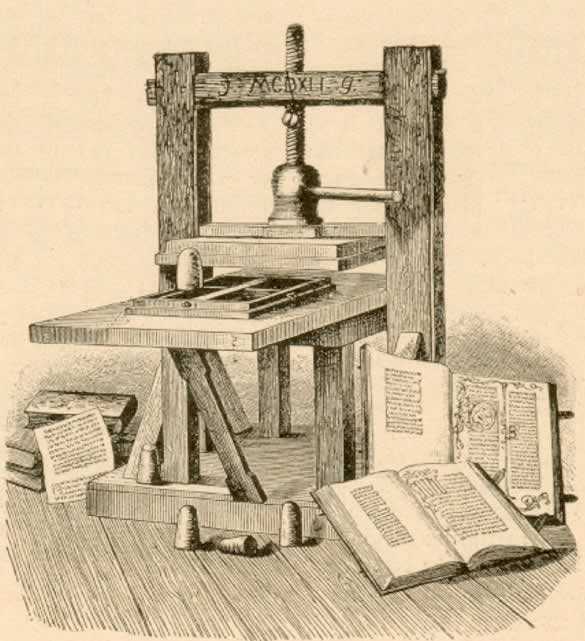
\includegraphics[width=0.7\textwidth]{images/presse} 
\caption[Druckerpresse von Gutenberg \cite{fig:presse}]{Druckerpresse von Gutenberg}
\label{fig:druckerpresse}
\end{figure}

Das Buch wurde zum Massenprodukt und damit zum Katalysator der Wissensgesellschaft die in logischer Konsequenz zur heutigen Informationsgesellschaft f"uhrte.


%%% Local Variables: 
%%% mode: latex
%%% TeX-master: "thesis"
%%% End: 
